\documentclass[11pt,a4paper]{ltjsarticle}

% LuaLaTeX用日本語パッケージ
\usepackage{luatexja}
\usepackage{luatexja-fontspec}

% 数学パッケージ
\usepackage{amsmath,amssymb,amsthm}
\usepackage{mathtools}

% 図式作成
\usepackage{tikz}
\usepackage{tikz-cd}
\usetikzlibrary{arrows,positioning,shapes}

% その他
\usepackage{hyperref}
\usepackage{enumitem}
\usepackage{geometry}
\usepackage{listings}
\usepackage{xcolor}

\geometry{margin=25mm}

% 定理環境
\theoremstyle{definition}
\newtheorem{definition}{定義}[section]
\newtheorem{theorem}[definition]{定理}
\newtheorem{lemma}[definition]{補題}
\newtheorem{proposition}[definition]{命題}
\newtheorem{example}[definition]{例}
\newtheorem{remark}[definition]{注意}

% Leanコード用スタイル
\lstdefinestyle{leanstyle}{
  language=ML,
  basicstyle=\ttfamily\small,
  keywordstyle=\color{blue}\bfseries,
  commentstyle=\color{green!60!black},
  stringstyle=\color{red},
  numbers=left,
  numberstyle=\tiny\color{gray},
  breaklines=true,
  frame=single,
  tabsize=2
}

\title{階数による停止性理論の形式化\\
  {\large ランク関数を用いた整礎性の証明}}
\author{
  TeXファイル生成: Claude Code\\
  Leanコード生成: Codex (OpenAI)
}
\date{\today}

\begin{document}

\maketitle

\begin{abstract}
本稿では、自然数への階数関数を用いた停止性証明の理論をLean 4で形式化した結果について解説する。
主要な定理は、型$X$上の関係$R$が自然数値ランク関数によって厳密に減少するならば、
$R$は整礎的(well-founded)であるという基本原理である。
この理論カーネルを実装し、リストの長さと整数の絶対値という2つの具体例で再利用可能性を実証した。
\end{abstract}

\tableofcontents

\section{導入}

プログラムの停止性を証明する基本的な手法の一つは、\textbf{ランク関数}(rank function)を用いることである。
実行ステップごとに厳密に減少する自然数値の測度を見つけることができれば、
無限降下列が存在しないことから、プログラムの停止性が保証される。

本稿では、この基本原理をLean 4で形式化し、以下を達成する：
\begin{enumerate}
\item 階数による整礎性の一般的な定理の証明（カーネル部分）
\item ステップ関数の停止性証明への応用
\item 具体例による再利用可能性の実証
\end{enumerate}

\section{基本概念}

\subsection{整礎関係}

\begin{definition}[整礎関係]
型$X$上の二項関係$R \subseteq X \times X$が\textbf{整礎的}(well-founded)であるとは、
$R$に関する無限降下列が存在しないことをいう。すなわち、
\[
x_0 \mathrel{R} x_1 \mathrel{R} x_2 \mathrel{R} \cdots
\]
となる列$\{x_n\}_{n \in \mathbb{N}}$が存在しない。
\end{definition}

整礎性は、Leanでは帰納的に定義される$\mathrm{Acc}$(accessible)述語と$\mathrm{WellFounded}$型クラスで表現される。

\subsection{ランク付き型}

\begin{definition}[ランク付き型]
型$X$と自然数への関数$r : X \to \mathbb{N}$の組$(X, r)$を\textbf{ランク付き型}と呼ぶ。
Leanでは、構造体$\texttt{Ranked Nat X}$として実装される：
\begin{lstlisting}[style=leanstyle]
structure Ranked (N : Type) (X : Type) where
  rank : X → N
\end{lstlisting}
\end{definition}

\section{主要定理：階数による整礎性}

\subsection{階数降下関係}

\begin{definition}[階数降下関係 $\mathrm{Desc}_R$]
\label{def:desc}
ランク付き型$(X, r)$に対して、\textbf{階数降下関係}$\mathrm{Desc}_R : X \to X \to \mathrm{Prop}$を
\[
\mathrm{Desc}_R(x, y) \;:\!\!\iff\; r(x) < r(y)
\]
と定義する。
\end{definition}

この関係は、Leanでは次のように実装される：
\begin{lstlisting}[style=leanstyle]
def Desc : X → X → Prop :=
  fun x y => R.rank x < R.rank y
\end{lstlisting}

\subsection{整礎性定理}

\begin{theorem}[階数降下関係の整礎性]
\label{thm:wf-desc}
任意のランク付き型$(X, r)$に対して、階数降下関係$\mathrm{Desc}_R$は整礎的である。
\end{theorem}

\begin{proof}
自然数上の標準的な順序$<$は整礎的である。
ランク関数$r : X \to \mathbb{N}$によって、この整礎性を$X$に引き戻すことができる。
具体的には、Mathlibの$\texttt{measure}$構成を用いる：
\[
\texttt{measure}\;r \;=\; \{(x, y) \mid r(x) < r(y)\} \;=\; \mathrm{Desc}_R
\]
したがって、$(\texttt{measure}\;r).\texttt{wf}$により整礎性が得られる。

Leanでの証明は1行：
\begin{lstlisting}[style=leanstyle]
theorem wf_desc : WellFounded (Desc (R := R)) := by
  simpa [Desc] using (measure R.rank).wf
\end{lstlisting}
\end{proof}

\begin{figure}[htbp]
\centering
\begin{tikzpicture}[node distance=2cm]
  % ノード
  \node (X) {$X$};
  \node (N) [right=of X] {$\mathbb{N}$};
  \node (WFX) [below=of X] {$\mathrm{WF}(\mathrm{Desc}_R)$};
  \node (WFN) [below=of N] {$\mathrm{WF}(<)$};

  % 矢印
  \draw[->] (X) -- node[above] {$r$} (N);
  \draw[->] (WFN) -- node[below] {引き戻し} (WFX);
  \draw[->] (N) -- node[right] {既知} (WFN);
  \draw[->] (X) -- node[left] {導出} (WFX);
\end{tikzpicture}
\caption{ランク関数による整礎性の引き戻し}
\label{fig:pullback}
\end{figure}

\subsection{一般化：任意の関係への適用}

\begin{theorem}[ランク減少による整礎性]
\label{thm:wf-rank-decreasing}
型$X$上の関係$R$とランク付き型$(X, r)$が与えられたとき、
\[
\forall x, y \in X,\quad R(x, y) \implies r(x) < r(y)
\]
ならば、$R$は整礎的である。
\end{theorem}

\begin{proof}
仮定より、$R \subseteq \mathrm{Desc}_R$である。
定理\ref{thm:wf-desc}より$\mathrm{Desc}_R$は整礎的であり、
部分関係の整礎性は保存されるため、$R$も整礎的である。
\end{proof}

\begin{figure}[htbp]
\centering
\begin{tikzcd}
X \times X \arrow[r, "R"] \arrow[rd, "\mathrm{Desc}_R"'] & \mathrm{Prop} \\
                                                         & \mathrm{WF} \arrow[u]
\end{tikzcd}
\caption{部分関係による整礎性の継承}
\end{figure}

\section{ステップ関数の停止性}

\subsection{ランク減少条件}

プログラムの1ステップ実行を関数$\mathrm{step} : X \to X$でモデル化する。

\begin{definition}[ランク減少]
\label{def:rank-decreases}
ステップ関数$\mathrm{step}$が$R = (X, r)$に関して\textbf{ランクを減少させる}とは、
\[
\forall x \in X,\quad r(\mathrm{step}(x)) < r(x)
\]
が成り立つことをいう。Leanでは：
\begin{lstlisting}[style=leanstyle]
structure RankDecreases {X : Type u}
    (R : Ranked Nat X) (step : X → X) : Prop where
  dec : ∀ x : X, R.rank (step x) < R.rank x
\end{lstlisting}
\end{definition}

\subsection{ステップ関係}

\begin{definition}[ステップ関係]
ステップ関数$\mathrm{step} : X \to X$から誘導される\textbf{ステップ関係}$\mathrm{StepRel}$を
\[
\mathrm{StepRel}(x, y) \;:\!\!\iff\; x = \mathrm{step}(y)
\]
と定義する。
\end{definition}

これは「$x$は$y$の次の状態である」という関係を表す。

\begin{theorem}[ステップ関係の整礎性]
\label{thm:wf-steprel}
$\mathrm{step}$がランクを減少させるならば、$\mathrm{StepRel}$は整礎的である。
したがって、無限実行列
\[
x_0, \;\mathrm{step}(x_0), \;\mathrm{step}^2(x_0), \;\ldots
\]
は存在しない。すなわち、どの初期状態$x_0$から始めても、プログラムは有限ステップで停止する。
\end{theorem}

\begin{proof}
定理\ref{thm:wf-rank-decreasing}を適用する。
$\mathrm{StepRel}(x, y)$ならば$x = \mathrm{step}(y)$であり、
定義\ref{def:rank-decreases}より$r(x) = r(\mathrm{step}(y)) < r(y)$である。
したがって、$\mathrm{StepRel} \subseteq \mathrm{Desc}_R$であり、整礎性が従う。
\end{proof}

\begin{figure}[htbp]
\centering
\begin{tikzpicture}[node distance=1.5cm and 3cm]
  % 状態の列
  \node (x0) {$x_0$};
  \node (x1) [right=of x0] {$x_1$};
  \node (x2) [right=of x1] {$x_2$};
  \node (dots) [right=of x2] {$\cdots$};

  % ランクの列
  \node (r0) [below=of x0] {$r_0$};
  \node (r1) [below=of x1] {$r_1$};
  \node (r2) [below=of x2] {$r_2$};
  \node (rdots) [below=of dots] {$\cdots$};

  % ステップ関係
  \draw[->] (x0) -- node[above] {$\mathrm{step}$} (x1);
  \draw[->] (x1) -- node[above] {$\mathrm{step}$} (x2);
  \draw[->] (x2) -- node[above] {$\mathrm{step}$} (dots);

  % ランク関数
  \draw[|->] (x0) -- node[left] {$r$} (r0);
  \draw[|->] (x1) -- (r1);
  \draw[|->] (x2) -- (r2);

  % ランクの減少
  \draw[->] (r1) -- node[above] {$<$} (r0);
  \draw[->] (r2) -- node[above] {$<$} (r1);
  \draw[->] (rdots) -- node[above] {$<$} (r2);

  % 矛盾の指摘
  \node (contra) [below=1.5cm of r1] {$\mathbb{N}$に無限降下列は存在しない！};
  \draw[red, thick, ->] (rdots) -- (contra);
\end{tikzpicture}
\caption{ステップ関数の停止性：自然数の無限降下列は不可能}
\label{fig:termination}
\end{figure}

\section{具体例による検証}

理論カーネルの再利用可能性を実証するため、2つの具体例を示す。

\subsection{例1：リストの末尾削除}

\begin{example}[リストの長さによる停止性]
型$A$に対して、$X = \mathrm{List}(A)$とし、ランク関数を
\[
r(xs) = \mathrm{length}(xs)
\]
と定める。\textbf{末尾削除関係}$\mathrm{TailRel}$を
\[
\mathrm{TailRel}(xs, ys) \;:\!\!\iff\; \exists a \in A,\; ys = a :: xs
\]
と定義する。すなわち、$xs$は$ys$の先頭要素を除いたものである。
\end{example}

\begin{proposition}
$\mathrm{TailRel}$は整礎的である。
\end{proposition}

\begin{proof}
$\mathrm{TailRel}(xs, ys)$ならば、ある$a$に対して$ys = a :: xs$である。このとき、
\[
r(xs) = \mathrm{length}(xs) < \mathrm{length}(a :: xs) = \mathrm{length}(ys) = r(ys)
\]
が成り立つ。定理\ref{thm:wf-rank-decreasing}より、$\mathrm{TailRel}$は整礎的である。

Lean実装：
\begin{lstlisting}[style=leanstyle]
def TailRel : List α → List α → Prop :=
  fun x y => ∃ a, y = a :: x

theorem wf_tailRel : WellFounded (TailRel (α := α)) := by
  let R : Ranked Nat (List α) := instRankedList
  refine wf_of_rank_decreasing (R := R)
                                (r := TailRel) ?_
  intro x y h
  rcases h with ⟨a, rfl⟩
  exact Nat.lt_succ_self (List.length x)
\end{lstlisting}
\end{proof}

\begin{figure}[htbp]
\centering
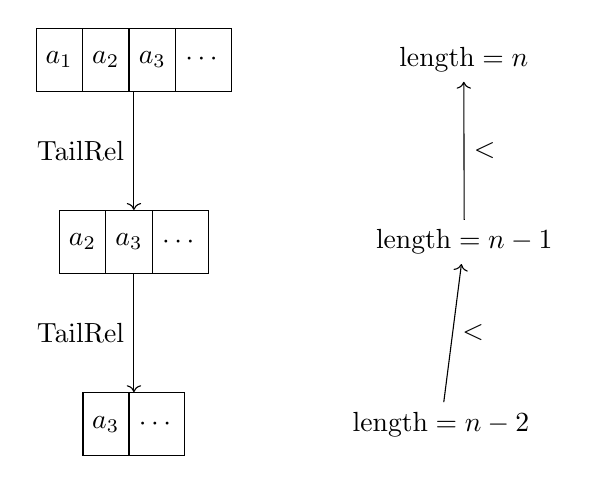
\begin{tikzpicture}[
  list/.style={rectangle split, rectangle split parts=#1,
               rectangle split horizontal, draw, minimum height=0.8cm},
  node distance=0.5cm
]
  \node[list=4] (l3) {$a_1$ \nodepart{two} $a_2$ \nodepart{three} $a_3$ \nodepart{four} $\cdots$};
  \node[list=3, below=1.5cm of l3] (l2) {$a_2$ \nodepart{two} $a_3$ \nodepart{three} $\cdots$};
  \node[list=2, below=1.5cm of l2] (l1) {$a_3$ \nodepart{two} $\cdots$};

  \node[right=2cm of l3] (r3) {$\mathrm{length} = n$};
  \node[right=2cm of l2] (r2) {$\mathrm{length} = n-1$};
  \node[right=2cm of l1] (r1) {$\mathrm{length} = n-2$};

  \draw[->] (l3) -- node[left] {$\mathrm{TailRel}$} (l2);
  \draw[->] (l2) -- node[left] {$\mathrm{TailRel}$} (l1);

  \draw[->] (r2) -- node[right] {$<$} (r3);
  \draw[->] (r1) -- node[right] {$<$} (r2);
\end{tikzpicture}
\caption{リストの末尾削除とランクの減少}
\end{figure}

\subsection{例2：整数の絶対値による降下}

\begin{example}[絶対値降下関係]
$X = \mathbb{Z}$（整数）とし、ランク関数を
\[
r(x) = |x|
\]
と定める（Leanでは$\texttt{Int.natAbs} : \mathbb{Z} \to \mathbb{N}$）。
\textbf{絶対値降下関係}$\mathrm{AbsDesc}$を
\[
\mathrm{AbsDesc}(x, y) \;:\!\!\iff\; |x| < |y|
\]
と定義する。
\end{example}

\begin{proposition}
$\mathrm{AbsDesc}$は整礎的である。
\end{proposition}

\begin{proof}
$\mathrm{AbsDesc}(x, y)$の定義は$r(x) < r(y)$に他ならない。
したがって、$\mathrm{AbsDesc} = \mathrm{Desc}_R$であり、
定理\ref{thm:wf-desc}より整礎的である。

Lean実装：
\begin{lstlisting}[style=leanstyle]
def AbsDesc : ℤ → ℤ → Prop :=
  fun x y => Int.natAbs x < Int.natAbs y

theorem wf_absDesc : WellFounded AbsDesc := by
  let R : Ranked Nat ℤ := instRankedInt
  refine wf_of_rank_decreasing (R := R)
                                (r := AbsDesc) ?_
  intro x y h
  exact h
\end{lstlisting}
\end{proof}

\begin{figure}[htbp]
\centering
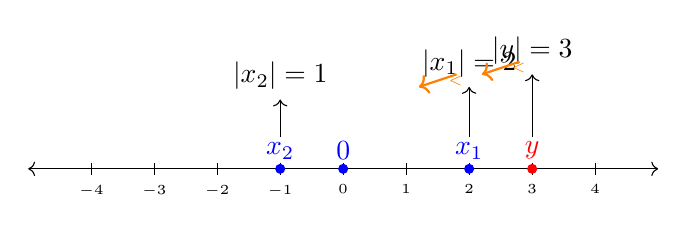
\begin{tikzpicture}[scale=0.8]
  % 数直線
  \draw[<->] (-5,0) -- (5,0);
  \foreach \x in {-4,-3,-2,-1,0,1,2,3,4}
    \draw (\x,0.1) -- (\x,-0.1) node[below] {\tiny$\x$};

  % 点の列
  \filldraw[red] (3,0) circle (2pt) node[above] {$y$};
  \filldraw[blue] (2,0) circle (2pt) node[above] {$x_1$};
  \filldraw[blue] (-1,0) circle (2pt) node[above] {$x_2$};
  \filldraw[blue] (0,0) circle (2pt) node[above] {$0$};

  % 絶対値の矢印
  \draw[->] (3,0.5) -- (3,1.5) node[above] {$|y|=3$};
  \draw[->] (2,0.5) -- (2,1.3) node[above] {$|x_1|=2$};
  \draw[->] (-1,0.5) -- (-1,1.1) node[above] {$|x_2|=1$};

  % 関係の矢印
  \draw[->, thick, orange] (2.8,1.7) -- (2.2,1.5) node[midway, right] {\tiny$<$};
  \draw[->, thick, orange] (1.8,1.5) -- (1.2,1.3) node[midway, right] {\tiny$<$};
\end{tikzpicture}
\caption{整数上の絶対値降下関係：$|x| < |y|$による整礎性}
\end{figure}

\section{理論カーネルの設計原理}

\subsection{最小性}

本形式化は意図的に\textbf{最小限}に保たれている：
\begin{itemize}
\item 依存するのは自然数$\mathbb{N}$上の整礎性のみ
\item より一般的な整礎順序への拡張は行わない
\item 証明は$\texttt{measure}$構成の1行の簡約
\end{itemize}

この設計により、理論カーネルは：
\begin{enumerate}
\item 理解しやすい
\item リファクタリングに強い
\item 依存関係が少ない
\end{enumerate}

\subsection{再利用可能性}

2つの例（リストと整数）が示すように、カーネル定理を適用する手順は機械的である：
\begin{enumerate}
\item 対象の型$X$に適切なランク関数$r : X \to \mathbb{N}$を定義
\item 目的の関係$R$がランクを減少させることを示す
\item 定理\ref{thm:wf-rank-decreasing}を適用
\end{enumerate}

各例の証明は数行で完了し、\textbf{整礎性のボイラープレートを排除}している。

\subsection{拡張性}

現在の実装は自然数ランクに限定されているが、将来的には：
\begin{itemize}
\item 順序数への拡張
\item 辞書式順序の組み込み
\item 相互再帰関数への応用
\end{itemize}
などが考えられる。しかし、基本カーネルは安定しており、これらは追加レイヤーとして実装できる。

\section{結論}

本稿では、自然数値ランク関数による停止性証明の理論をLean 4で形式化した。
主要な成果は：

\begin{enumerate}
\item \textbf{カーネル定理}：階数降下関係$\mathrm{Desc}_R$の整礎性（定理\ref{thm:wf-desc}）
\item \textbf{応用定理}：ランク減少による一般関係の整礎性（定理\ref{thm:wf-rank-decreasing}）
\item \textbf{実用例}：リストと整数における停止性証明
\end{enumerate}

この形式化は、\textbf{最小性}、\textbf{再利用可能性}、\textbf{拡張性}の3つの設計原理に基づいており、
形式的証明支援系における停止性証明の実用的な基盤となる。

\subsection{貢献の明示}

\begin{itemize}
\item \textbf{Leanコード生成}：Codex (OpenAI) により、基本的な証明構造と定理記述が生成された。
\item \textbf{TeX文書生成}：Claude Code により、本稿の日本語による数学的解説と図式が生成された。
\item 両者の協働により、形式証明とその解説の統合的な文書化が実現された。
\end{itemize}

\appendix

\section{Leanコード全文}

参考のため、実装の全体を示す：

\begin{lstlisting}[style=leanstyle]
import Mathlib
import MyProjects.ST.RankCore.Basic
import MyProjects.ST.RankCore.P3.ListLength
import MyProjects.ST.RankCore.P3.IntAbs

/-!
Termination via rank.

Key defs: `Desc`, `StepRel`.
Key lemmas: `wf_desc`, `wf_of_rank_decreasing`,
            `wf_stepRel`, `acc_of_rank`.
-/

namespace ST

open scoped Classical

universe u v

/-- A step relation decreases rank. -/
structure RankDecreases {X : Type u}
    (R : Ranked Nat X) (step : X → X) : Prop where
  dec : ∀ x : X, R.rank (step x) < R.rank x

namespace Termination

variable {X : Type u} (R : Ranked Nat X) (step : X → X)

/-- The "rank-descending" relation induced by R. -/
def Desc : X → X → Prop :=
  fun x y => R.rank x < R.rank y

/-- Well-foundedness of Desc. -/
theorem wf_desc : WellFounded (Desc (R := R)) := by
  simpa [Desc] using (measure R.rank).wf

theorem wf_of_rank_decreasing (r : X → X → Prop)
    (h : ∀ {x y}, r x y → R.rank x < R.rank y) :
    WellFounded r := by
  refine (wf_desc (R := R)).mono ?_
  intro x y hxy
  exact h hxy

def StepRel : X → X → Prop :=
  fun x y => x = step y

theorem wf_stepRel (hdec : RankDecreases R step) :
    WellFounded (StepRel (step := step)) := by
  refine wf_of_rank_decreasing (R := R)
                                (r := StepRel) ?_
  intro x y hxy
  subst hxy
  exact hdec.dec y

theorem acc_of_rank (x : X) : Acc (Desc (R := R)) x :=
  (wf_desc (R := R)).apply x

end Termination

/-! ## Examples -/

section Examples

open Termination

variable {α : Type u}

def TailRel : List α → List α → Prop :=
  fun x y => ∃ a, y = a :: x

theorem wf_tailRel : WellFounded (TailRel (α := α)) := by
  let R : Ranked Nat (List α) := instRankedList
  refine wf_of_rank_decreasing (R := R)
                                (r := TailRel) ?_
  intro x y h
  rcases h with ⟨a, rfl⟩
  exact Nat.lt_succ_self (List.length x)

def AbsDesc : ℤ → ℤ → Prop :=
  fun x y => Int.natAbs x < Int.natAbs y

theorem wf_absDesc : WellFounded AbsDesc := by
  let R : Ranked Nat ℤ := instRankedInt
  refine wf_of_rank_decreasing (R := R)
                                (r := AbsDesc) ?_
  intro x y h
  exact h

end Examples

end ST
\end{lstlisting}

\end{document}
